\section{Different forms of games}\label{sec:game_theory_intro}

In game theory there are several different forms of games.
In this section we will outline only the ones necessary for the formulation
of the scenario studied in this research project.
The first one is normal form games the second one is perfect information
extensive form games and the third one is extensive form games with imperfect
information.


\subsection{Normal form games}\label{sec:intro_normal_form_games}

Normal form games are strategic games that model strategic decision-makers.
These decision makers are referred to as players where each player has a
set of possible actions that they can take.
The game captures the interaction between the players by taking into account
the payoffs that each player receives for each possible combination of actions
taken by all players.
A strategic game consists of a set of players, a set of actions for each player,
and a payoff function that maps each combination of actions to a payoff for
each player~\cite{osborne2004_normal_form_games}.

Normal form games with \(n\) players are usually represented by \(n\)
matrices that include the payoffs for each player for every possible combination
of actions.
A 2-player normal form game is represented by two matrices \(A\) (for player 1)
and \(B\) (for player 2) where the rows of each matrix correspond to the actions
of player 1 and the columns of each matrix correspond to the actions of player
2.
For example, consider the Prisoner's Dilemma game shown in
Table~\ref{tab:prisoners_dilemma}.
In this game, player 1 can choose to either cooperate or defect and player 2
can also choose to either cooperate or defect.
The payoff matrix \(A\) shows the payoffs for player 1 and the payoff matrix
\(B\) shows the payoffs for player 2.

\begin{table}[H]
    \centering
    \caption{The Prisoner's Dilemma game}
    \begin{tabular}{|c|c|c|}
        \hline
        \backslashbox{Player 1}{Player 2} & Cooperate & Defect \\
        \hline
        Cooperate & \(3,3\) & \(0,5\) \\
        \hline
        Defect & \(5,0\) & \(1,1\) \\
        \hline
    \end{tabular}
    \label{tab:prisoners_dilemma}
\end{table}

The entry in the first row and first column of table~\ref{tab:prisoners_dilemma}
is \(3,3\).
That indicates that if both players choose to cooperate then they both receive
a payoff of 3.
Similarly the entry in the second row and first column is \(0,5\).
That indicates that if player 1 chooses to defect and player 2 chooses to
cooperate then player 1 receives a payoff of 0 and player 2 receives a payoff
of 5.

Equivalently, a 3-player normal form game is represented by three matrices
\(A\), \(B\) and \(C\) where the rows of each matrix correspond to the actions
of player 1, the columns of each matrix correspond to the actions of player 2
and the third dimension of each matrix corresponds to the actions of player 3.

% TODO: Do I need a subsection on Nash equilibrium here?
% TODO: If yes, do I need one on learning algorithms as well?
% TODO: If yes, do I need one specific on asymmetric replicator dynamics?



\subsection{Perfect-information extensive form game}

Strategic games like normal form games suppress the sequential nature of most
decision-making situations.
There are numerous situations where decision makers can change their actions
based on the actions of other decision makers.
Such type of sequential games are also referred to as extensive form games.
One of the most common types of extensive form games is the perfect-information
extensive form game.
In this type of game, the players are assumed to have perfect information
about the previous actions of other
players.
There are four key components of a perfect-information extensive form game; the
players, the terminal nodes, the player function and the preferences of the
players~\cite{osborne2004_extensive_form_games}.
Examples of such games are the game of chess and the game of
Backgammon~\cite{hart1992games}.

Perfect information extensive form games are represented by a tree where the
nodes of the tree are the terminal nodes and represent the outcome of the
game.
The following figure shows an example of a perfect information extensive form
game.

\begin{figure}[H]
    \centering
    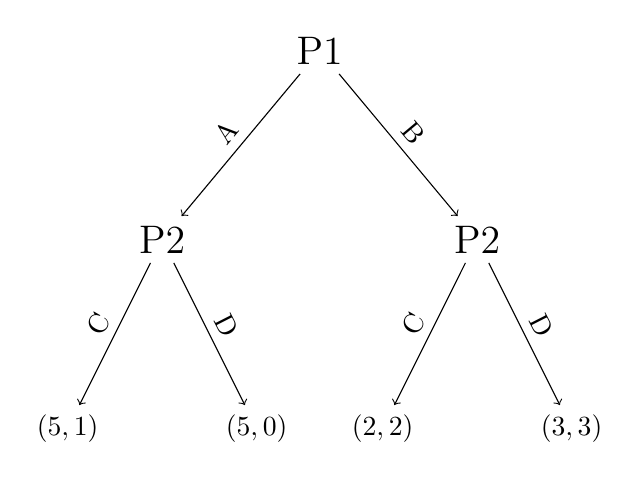
\begin{tikzpicture}[-, node distance = 2cm, scale=0.8]
    \node[anchor=north](P1){\Large{P1}};
    \node[anchor=north](P2_1) at (-2.5, -3) {\Large{P2}};
    \node[anchor=north](P2_2) at (2.5, -3) {\Large{P2}};

    \path[->] (P1) edge node [above, rotate=50] {A}(P2_1);
    \path[<-] (P2_2) edge node [above, rotate=310] {B}(P1);

    \node[anchor=north](F_1) at (-4, -6) {\((5,1)\)};
    \node[anchor=north](F_2) at (-1, -6) {\((5,0)\)};
    \node[anchor=north](F_3) at (1, -6) {\((2,2)\)};
    \node[anchor=north](F_4) at (4, -6) {\((3,3)\)};

    \path[->] (P2_1) edge node [above, rotate=60] {C}(F_1);
    \path[->] (P2_1) edge node [above, rotate=297] {D}(F_2);
    \path[->] (P2_2) edge node [above, rotate=60] {C}(F_3);
    \path[->] (P2_2) edge node [above, rotate=297] {D}(F_4);
\end{tikzpicture}

    \caption{An example of a perfect information extensive form game}
    \label{fig:extensive_form_game}
\end{figure}

Figure~\ref{fig:extensive_form_game} shows an example of a perfect information
extensive form game.
The game starts at the root node and the players take turns to make a move.
Player 1 can choose to either action A or action B.
Once player 1 has made a move, player 2 can choose to either action C or action
D, while having complete awareness of the action taken by player 1 and hence
their own position on the tree.
The final nodes of the tree represent the outcome of the game.
In this example, the outcome of the game is either 

\subsection{Imperfect-information extensive form game}
\label{sec:game_imperfect_information}

An imperfect information game is defined as an extensive form game where some
of the information about the game state is hidden for at least one of the
players~\cite{Berwanger2008}.
In other words, when making a decision, the players might not know their exact
position on the tree.
Similar to perfect information, imperfect information games are also represented
by a tree.
The following figure shows an example of an imperfect information extensive
form game.

\begin{figure}[H]
    \centering
    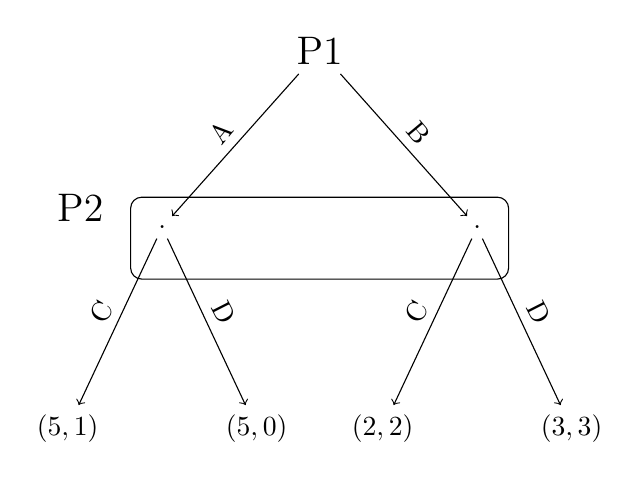
\begin{tikzpicture}[-, node distance = 2cm, scale=0.8]
    \node[anchor=north](P1){\Large{P1}};
    \node[anchor=north](P2_1) at (-2.5, -3) {.};
    \node[anchor=north](P2_2) at (2.5, -3) {.};
    \node[anchor=north](P2_3) at (-3.8, -2.5) {\Large{P2}};

    % \draw (0,-3.4) ellipse (3cm and 1cm);
    \draw[rounded corners] (-3, -4) rectangle (3, -2.7) {};

    \path[->] (P1) edge node [above, rotate=50] {A}(P2_1);
    \path[<-] (P2_2) edge node [above, rotate=310] {B}(P1);

    \node[anchor=north](F_1) at (-4, -6) {\((5,1)\)};
    \node[anchor=north](F_2) at (-1, -6) {\((5,0)\)};
    \node[anchor=north](F_3) at (1, -6) {\((2,2)\)};
    \node[anchor=north](F_4) at (4, -6) {\((3,3)\)};

    \path[->] (P2_1) edge node [above, rotate=60] {C}(F_1);
    \path[->] (P2_1) edge node [above, rotate=297] {D}(F_2);
    \path[->] (P2_2) edge node [above, rotate=60] {C}(F_3);
    \path[->] (P2_2) edge node [above, rotate=297] {D}(F_4);
\end{tikzpicture}

    \caption{An example of a perfect information extensive form game}
    \label{fig:imperfect_extensive_form_game}
\end{figure}

Figure~\ref{fig:imperfect_extensive_form_game} shows an example of an imperfect
information extensive form game where player 2, when making their decision,
does not know whether they are in the left or right branch of the tree.
The game starts at the root node and the players take turns to make a move.
Player 1 can choose to either action A or action B.
Once player 1 has made a move, player 2 can choose to either action C or action
D, while having incomplete awareness of the action taken by player 1 and hence
their own position on the tree.
The final nodes of the tree represent the outcome of the game.
This game can also be represented by a normal form game since both players end
up being completely unaware of the actions taken by the other player.
Table~\ref{tab:imperfect_to_normal_form} shows the normal form game
representation of the imperfect information extensive form game shown in
Figure~\ref{fig:imperfect_extensive_form_game}.


\begin{table}[H]
    \centering
    \caption{Normal-form representation of imperfect information
    extensive-form game}
    \begin{tabular}{|c|c|c|}
        \hline
        \backslashbox{Player 1}{Player 2} & C & D \\
        \hline
        A & \(5,1\) & \(5,0\) \\
        \hline
        B & \(2,2\) & \(3,3\) \\
        \hline
    \end{tabular}
    \label{tab:imperfect_to_normal_form}
\end{table}